\section{Aufbau und Durchführung}

Der generelle Aufbau des Geiger-Müller-Zählrohrs wurde bereits im vorherigen Kapitel erläutert. Wie in Abbildung \ref{fig:schaltbild} zu sehen ist, fließt die Ladung $Q$, die sich am Anodendraht sammelt, über den Widerstand $R$ und kann dann über einen 
Kondensator $C$ und einen Verstärker als Spannungsimpuls gemessen werden. Dieser kann auch über einen Oszillographen dargestellt werden.


\begin{figure}[h!tbp]
	\centering
	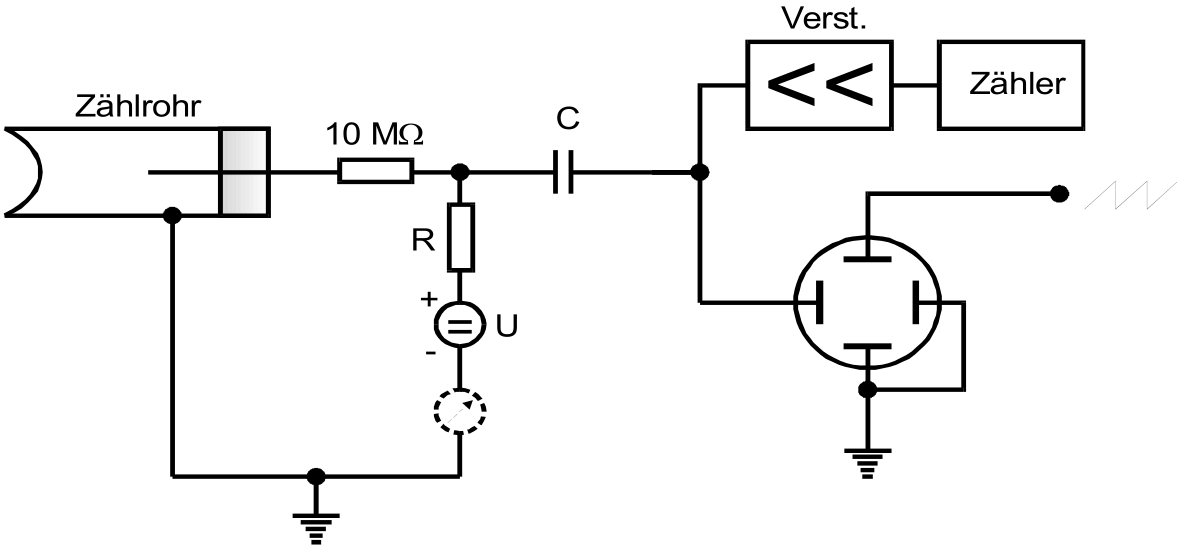
\includegraphics[width=0.7\linewidth]{schaltbild.png}
	\caption{Skizze der Messapparatur.\cite[7]{anleitung703}}
	\label{fig:schaltbild}
\end{figure}

In diesem Versuch soll zunächst die Charakteristik des Zählrohrs aufgenommen werden. Dazu wird ein $\beta$-Strahler vor dem Zählrohr platziert. In 10\,V-Schritten werden für Spannungen zwischen 300 und 700\,V für jeweils 60\,s die Zählraten gemessen 
und gegeneinander aufgetragen.

Desweiteren können mithilfe des Oszilloskops die Nachentladungen, die für den Anstieg des Plateaus sorgen, dargestellt werden. Da es aus technischen Gründen nicht möglich ist, die Bilder auf dem Oszilloskop genauer zu analysieren, soll der Verlauf der
zu beobachtenden Kurve nur qualitativ erklärt werden.

Zudem soll die Totzeit auf zwei verschiedene Weisen gemessen werden. Die erste Messung erfolgt über das Oszilloskop. Dazu wird die Kurve so verschoben, dass mithilfe des Gitters und den Einstellungen am Oszilloskop die Totzeit abgelesen und die 
Erholungszeit grob abgeschätzt werden kann. Für die andere Methode wird eine zweite Strahlungsquelle eingesetzt, es handelt sich also um die sogenannte Zwei-Quellen-Methode. Die Grundlage hierfür ist wahre Impulsrate $N_{\text{w}}$ der eindringenden und absorbierten
Teilchen pro Zeiteinheit. Sie ist gegeben durch die registrierte Impulsrate $N_{\text{r}}$. $TN_{\text{r}}$ ist hierbei der Bruchteil der Messzeit, für die das Zählrohr unempfindlich ist:

\begin{equation}
N_{\text{w}} = \frac{\text{Impulsrate}}{\text{Messzeit}} = \frac{N_{\text{r}} \cdot t}{(1-TN_{\text{r}})\cdot t} = \frac{N_{\text{r}}}{1-TN_{\text{r}}}
\label{eqn:impulsrate}
\end{equation}
Im Experiment wird zunächst die Zählrate $N_1$ des ersten Präparats gemessen. Im Anschluss wird ein zweites Präparat hinzugefügt um die Zählrate $N_{1+2}$ beider Präparate zusamamen zu messen, wobei darauf geachtet wird, dass das erste Präparat nicht bewegt wird.
Zuletzt wird das erste Präparat wieder aus der Halterung genommen und nur die Zählrate $N_2$ des zweiten Präparates gemessen. Aus \ref{eqn:impulsrate} ergeben sich dann die folgenden Gleichungen:

\begin{equation}
\begin{aligned}
N_{\text{w,1}} &= \frac{N_1}{1 - TN_1}, \\
N_{\text{w,2}} &= \frac{N_2}{1 - TN_2}, \\
N_{\text{w,1+2}} &= \frac{N_{1+2}}{1 - TN_{1+2}}. \\
\end{aligned}
\end{equation}
Mit $N_{\text{w,1+2}} = N_{\text{w,1}} + N_{\text{w,2}}$ folgt:

\begin{equation}
\frac{N_{\text{w,1+2}}}{1 - TN_{\text{w,1+2}}} = \frac{N_1}{1 - TN_1} + \frac{N_2}{1 - TN_2}.
\label{eqn:gleichung}
\end{equation}
Da $N_1$, $N_2$ und $N_{1+2}$ messbare Größen sind, kann aus ihnen die Totzeit berechnet werden. Dazu kann Gleichung \ref{eqn:gleichung} näherungsweise zu

\begin{equation}
T \approx \frac{N_1 + N_2 - N_{1+2}}{2N_1 N_2}
\end{equation}
umgestellt werden.

Im letzten Teil des Versuchs wie die pro Teilchen am Zählrohr freigesetzte Ladungsmenge untersucht. Ist die Impulszahl pro Zeiteinheit bekannt, so kann die Ladungsmenge mithilfe des mittleren Zählrohrstroms $\bar{I}$:

\begin{equation}
\bar{I} \:= \frac{1}{\tau} \int_0^\tau \frac{U(t)}{R} \symup{d}t
\end{equation}
berechnet werden. Der Zählrohrstrom ist die transportierte Ladungsmenge $\Delta Q$ pro Zeitintervall $\Delta t$, während der $Z$ Teilchen registriert werden:

\begin{equation}
\bar{I} = \frac{\Delta Q}{\Delta t}\cdot Z.
\end{equation}
Dabei soll die Ladung $\Delta Q$ in Abhängigkeit von der Spannung $U$ gemessen werden.